% Options for packages loaded elsewhere
\PassOptionsToPackage{unicode}{hyperref}
\PassOptionsToPackage{hyphens}{url}
\PassOptionsToPackage{dvipsnames,svgnames,x11names}{xcolor}
%
\documentclass[
  a4paper,
]{article}

\usepackage{amsmath,amssymb}
\usepackage{iftex}
\ifPDFTeX
  \usepackage[T1]{fontenc}
  \usepackage[utf8]{inputenc}
  \usepackage{textcomp} % provide euro and other symbols
\else % if luatex or xetex
  \usepackage{unicode-math}
  \defaultfontfeatures{Scale=MatchLowercase}
  \defaultfontfeatures[\rmfamily]{Ligatures=TeX,Scale=1}
\fi
\usepackage{lmodern}
\ifPDFTeX\else  
    % xetex/luatex font selection
\fi
% Use upquote if available, for straight quotes in verbatim environments
\IfFileExists{upquote.sty}{\usepackage{upquote}}{}
\IfFileExists{microtype.sty}{% use microtype if available
  \usepackage[]{microtype}
  \UseMicrotypeSet[protrusion]{basicmath} % disable protrusion for tt fonts
}{}
\makeatletter
\@ifundefined{KOMAClassName}{% if non-KOMA class
  \IfFileExists{parskip.sty}{%
    \usepackage{parskip}
  }{% else
    \setlength{\parindent}{0pt}
    \setlength{\parskip}{6pt plus 2pt minus 1pt}}
}{% if KOMA class
  \KOMAoptions{parskip=half}}
\makeatother
\usepackage{xcolor}
\usepackage[top=2.54cm,right=2.54cm,bottom=2.54cm,left=2.54cm]{geometry}
\setlength{\emergencystretch}{3em} % prevent overfull lines
\setcounter{secnumdepth}{-\maxdimen} % remove section numbering
% Make \paragraph and \subparagraph free-standing
\makeatletter
\ifx\paragraph\undefined\else
  \let\oldparagraph\paragraph
  \renewcommand{\paragraph}{
    \@ifstar
      \xxxParagraphStar
      \xxxParagraphNoStar
  }
  \newcommand{\xxxParagraphStar}[1]{\oldparagraph*{#1}\mbox{}}
  \newcommand{\xxxParagraphNoStar}[1]{\oldparagraph{#1}\mbox{}}
\fi
\ifx\subparagraph\undefined\else
  \let\oldsubparagraph\subparagraph
  \renewcommand{\subparagraph}{
    \@ifstar
      \xxxSubParagraphStar
      \xxxSubParagraphNoStar
  }
  \newcommand{\xxxSubParagraphStar}[1]{\oldsubparagraph*{#1}\mbox{}}
  \newcommand{\xxxSubParagraphNoStar}[1]{\oldsubparagraph{#1}\mbox{}}
\fi
\makeatother


\providecommand{\tightlist}{%
  \setlength{\itemsep}{0pt}\setlength{\parskip}{0pt}}\usepackage{longtable,booktabs,array}
\usepackage{calc} % for calculating minipage widths
% Correct order of tables after \paragraph or \subparagraph
\usepackage{etoolbox}
\makeatletter
\patchcmd\longtable{\par}{\if@noskipsec\mbox{}\fi\par}{}{}
\makeatother
% Allow footnotes in longtable head/foot
\IfFileExists{footnotehyper.sty}{\usepackage{footnotehyper}}{\usepackage{footnote}}
\makesavenoteenv{longtable}
\usepackage{graphicx}
\makeatletter
\def\maxwidth{\ifdim\Gin@nat@width>\linewidth\linewidth\else\Gin@nat@width\fi}
\def\maxheight{\ifdim\Gin@nat@height>\textheight\textheight\else\Gin@nat@height\fi}
\makeatother
% Scale images if necessary, so that they will not overflow the page
% margins by default, and it is still possible to overwrite the defaults
% using explicit options in \includegraphics[width, height, ...]{}
\setkeys{Gin}{width=\maxwidth,height=\maxheight,keepaspectratio}
% Set default figure placement to htbp
\makeatletter
\def\fps@figure{htbp}
\makeatother

% Preámbulo
\usepackage{comment} % Permite comentar secciones del código
\usepackage{marvosym} % Agrega símbolos adicionales
\usepackage{graphicx} % Permite insertar imágenes
\usepackage{mathptmx} % Fuente de texto matemática
\usepackage{amssymb} % Símbolos adicionales de matemáticas
\usepackage{lipsum} % Crea texto aleatorio
\usepackage{amsthm} % Teoremas y entornos de demostración
\usepackage{float} % Control de posiciones de figuras y tablas
\usepackage{rotating} % Rotación de elementos
\usepackage{multirow} % Celdas combinadas en tablas
\usepackage{tabularx} % Tablas con ancho de columna ajustable
\usepackage{mdframed} % Marcos alrededor de elementos flotantes

% Series de tiempo
\usepackage{booktabs}


% Configuración adicional

\makeatletter
\@ifpackageloaded{caption}{}{\usepackage{caption}}
\AtBeginDocument{%
\ifdefined\contentsname
  \renewcommand*\contentsname{Tabla de contenidos}
\else
  \newcommand\contentsname{Tabla de contenidos}
\fi
\ifdefined\listfigurename
  \renewcommand*\listfigurename{Listado de Figuras}
\else
  \newcommand\listfigurename{Listado de Figuras}
\fi
\ifdefined\listtablename
  \renewcommand*\listtablename{Listado de Tablas}
\else
  \newcommand\listtablename{Listado de Tablas}
\fi
\ifdefined\figurename
  \renewcommand*\figurename{Figura}
\else
  \newcommand\figurename{Figura}
\fi
\ifdefined\tablename
  \renewcommand*\tablename{Tabla}
\else
  \newcommand\tablename{Tabla}
\fi
}
\@ifpackageloaded{float}{}{\usepackage{float}}
\floatstyle{ruled}
\@ifundefined{c@chapter}{\newfloat{codelisting}{h}{lop}}{\newfloat{codelisting}{h}{lop}[chapter]}
\floatname{codelisting}{Listado}
\newcommand*\listoflistings{\listof{codelisting}{Listado de Listados}}
\makeatother
\makeatletter
\makeatother
\makeatletter
\@ifpackageloaded{caption}{}{\usepackage{caption}}
\@ifpackageloaded{subcaption}{}{\usepackage{subcaption}}
\makeatother
\ifLuaTeX
\usepackage[bidi=basic]{babel}
\else
\usepackage[bidi=default]{babel}
\fi
\babelprovide[main,import]{spanish}
% get rid of language-specific shorthands (see #6817):
\let\LanguageShortHands\languageshorthands
\def\languageshorthands#1{}
\ifLuaTeX
  \usepackage{selnolig}  % disable illegal ligatures
\fi
\usepackage[]{biblatex}
\addbibresource{../../../references.bib}
\usepackage{bookmark}

\IfFileExists{xurl.sty}{\usepackage{xurl}}{} % add URL line breaks if available
\urlstyle{same} % disable monospaced font for URLs
\hypersetup{
  pdftitle={Notas de Clase Series de Tiempo},
  pdfauthor={Edison Achalma},
  pdflang={es},
  colorlinks=true,
  linkcolor={blue},
  filecolor={Maroon},
  citecolor={Blue},
  urlcolor={Blue},
  pdfcreator={LaTeX via pandoc}}

\title{Notas de Clase Series de Tiempo}
\usepackage{etoolbox}
\makeatletter
\providecommand{\subtitle}[1]{% add subtitle to \maketitle
  \apptocmd{\@title}{\par {\large #1 \par}}{}{}
}
\makeatother
\subtitle{Descubre cómo seleccionar hardware, descargar la imagen ISO y
preparar los medios de instalación. Exploraremos opciones para probar o
instalar Linux en tu equipo.}
\author{Edison Achalma}
\date{2023-08-27}

\begin{document}
\maketitle

\section{Modelos de Series de Tiempo
Estacionarias}\label{modelos-de-series-de-tiempo-estacionarias}

\subsection{Definición de ergodicidad y
estacionariedad}\label{definiciuxf3n-de-ergodicidad-y-estacionariedad}

A partir de esta sección introduciremos mayor formalidad matemática al
análisis, por ello cambiaremos de notación y ocuparemos a \(X_t\) en
lugar de \(Z_t\). Con \(X_t\) denotaremos a una serie de tiempo, ya que
con \(Z_t\) denotareemos a una variable, sin que ella fuera
necesariamente una serie de tiempo. Asimismo, iniciaremos por establecer
una serie de definiciones. De esta forma, definiremos a una serie de
tiempo como un vector de variables aleatorias de dimensión \(T\), dado
como:

\[
X_1, X_2, X_3, \ldots ,X_T
\]

Cada una de las \(X_t\) (\(t = 1, 2, \ldots, T\)) consideradas como una
variable aleatoria. Así, también podemos denotar a la serie de tiempo
como:

\begin{equation}\phantomsection\label{eq-Serie}{
\{ X_t \}^T_{t = 1}
}\end{equation}

Es decir, definiremos a una serie de tiempo como una realización de un
proceso estocástico --o un Proceso Generador de Datos (PGD).
Consideremos una muestra de los múlples posibles resultados de muestras
de tamaño \(T\), la colección dada por:

\[
\{X^{(1)}_1, X^{(1)}_2, \ldots, X^{(1)}_T\}
\]

es una de las tantas posibles resultantes del proceso estocástico o PGD.
Eventualmente podríamos estar dispuestos a observar este proceso
indefinidamente, de forma tal que estemos interesados en observar a la
secuencia dada por \(\{ X^{(1)}_t \}^{\infty}_{t = 1}\), lo cual no
dejaría se ser sólo una de las tantas realizaciones o secuencias del
proceso estocástico original.

Tan solo para poner un ejemplo, podríamos observar las siguientes
realizaciones del mismo PGD:

\begin{eqnarray*}
  & \{X^{(2)}_1, X^{(2)}_2, \ldots, X^{(2)}_T\} & \\
  & \{X^{(3)}_1, X^{(3)}_2, \ldots, X^{(3)}_T\} & \\
  & \{X^{(4)}_1, X^{(4)}_2, \ldots, X^{(4)}_T\} & \\
  & \vdots & \\
  & \{X^{(j)}_1, X^{(j)}_2, \ldots, X^{(j)}_T\} &
\end{eqnarray*}

Donde \(j \in \mathbb{Z}\). En lo subsecuente, diremos que una serie de
tiempo es una realización del proceso estocástico subyacente.
Considerando, en consecuencia, al proceso estocástico con todas sus
posibilidades de realización.

Para hacer más sencilla la notación no distinguiremos entre el proceso
en sí mismo y una de sus realizaciones, es decir, siempre escribiremos a
una serie de tiempo como la secuencia mostrada en la ecuación
(Ecuación~\ref{eq-Serie}), o más precisamente como la siguiente
realización:

\[
\{ X_1, X_2, \ldots, X_T \}
\]

O simplemente:

\[
X_1, X_2, \ldots, X_T
\]

El proceso estocástico de dimensión \(T\) puede ser completamente
descrito por su función de distribución multivaraida de dimensión \(T\).
No obstante, esto no resulta ser práctico cuando se opere más adelante
en el curso. Por ello, en el curso, y en general casi todos los textos
lo hacen, sólo nos enfocaremos en sus primer y segundo momentos, es
decir, en sus medias o valores esperados:

\[
\mathbb{E}[X_t]
\]

Para \(t = 1, 2, \ldots, T\); o:

\[
\left[
    \begin{array}{c}
    \mathbb{E}[X_1] \\
    \mathbb{E}[X_2] \\
    \vdots \\
    \mathbb{E}[X_T]
    \end{array}
\right]
\]

o,

\[
\left[
    \begin{array}{c}
    \mathbb{E}[X_1], \mathbb{E}[X_2], \ldots, \mathbb{E}[X_T]
    \end{array}
\right]
\]

De sus variazas:

\[
Var[X_t] = \mathbb{E}[(X_t - \mathbb{E}[X_t])^2]
\]

Para \(t = 1, 2, \ldots, T\), y de sus \(T(T-1)/2\) covarianzas:

\[
Cov[X_t,X_s] = \mathbb{E}[(X_t - \mathbb{E}[X_t])(X_s - \mathbb{E}[X_s])]
\]

Para \(t < s\). Por lo tanto, en la forma matricial podemos escribir lo
siguiente:

\[
\left[
    \begin{array}{c c c c}
    Var[X_1] & Cov[X_1,X_2] & \cdots & Cov[X_1,X_T] \\
    Cov[X_2,X_1] & Var[X_2] & \cdots & Cov[X_2,X_T] \\
    \vdots & \vdots & \ddots & \vdots \\
    Cov[X_T,X_1] & Cov[X_T,X_2] & \cdots & Var[X_T] \\
    \end{array}
\right]
\]

\begin{equation}\phantomsection\label{eq-MATCOV}{
= \left[
    \begin{array}{c c c c}
    \sigma_1^2 & \rho_{12} & \cdots & \rho_{1T} \\
    \rho_{21} & \sigma_2^2 & \cdots & \rho_{2T} \\
    \vdots & \vdots & \ddots & \vdots \\
    \rho_{T1} & \rho_{T2} & \cdots & \sigma_T^2 \\
    \end{array}
\right]
}\end{equation}

Donde es claro que en la matriz de la ecuación
(Ecuación~\ref{eq-MATCOV}) existen \(T(T-1)/2\) covarianzas distintas,
ya que se cumple que \(Cov[X_t,X_s] = Cov[X_s,X_t]\), para \(t \neq s\).

A menudo, esas covarianzas son denominadas como autocovarianzas puesto
que ellas son covarianzas entre variables aleatorias pertenecientes al
mismo proceso estocástico pero en un momento \(t\) diferente. Si el
proceso estocástico tiene una distribución normal multivariada, su
función de distribución estará totalmente descrita por sus momentos de
primer y segundo orden.

Ahora introduciremos el concepto de ergodicidad, el cual indica que los
momentos muestrales, los cuales son calculados en la base de una serie
de tiempo con un número finito de observaciones, en la medida que
\(T \rightarrow \infty\) sus correspondientes momentos muestrales,
tienden a los verdaderos valores poblacionales, los cuales definiremos
como \(\mu\), para la media, y \(\sigma^2_X\) para la varianza.

Este concepto sólo es cierto si asumimos que, por ejemplo, el valor
esperado y la varianza son como se dice a continuación para todo
\(t = 1, 2, \ldots, T\):

\begin{eqnarray}
    \mathbb{E}[X_t] = \mu_t = \mu \\
    \label{MEDIA}
    Var[X_t] = \sigma^2_X
\end{eqnarray} \{\#eq-VARIANZA\}

Mas formalmente, se dice que el PGD o el proceso estocástico es ergódico
en la media si:

\[
\displaystyle\lim_{T \to \infty}{\mathbb{E} \left[ \left( \frac{1}{T} \sum^{T}_{t = 1} (X_t - \mu) \right) ^2 \right]} = 0
\]

y ergódico en la varianza si:

\[
\displaystyle\lim_{T \to \infty}{\mathbb{E} \left[ \left( \frac{1}{T} \sum^{T}_{t = 1} (X_t - \mu) ^2 - \sigma^2_X \right) ^2 \right]} = 0
\]

Estas condiciones se les conoce como \emph{propiedades de consistencia}
para las variables aleatorias. Sin embargo, éstas no pueden ser
probadas. Por ello se les denomina como un supuesto que pueden cumplir
algunas de las series. Más importante aún: \textbf{un proceso
estocástico que tiende a estar en equilibrio estadístico en un orden
ergódico, es estacionario}.

Podemos distinguir dos tipos de estacionariedad. Si asumimos que la
función común de distribución del proceso estocástico no cambia a lo
largo del tiempo, se dice que el proceso es \emph{estrictamente
estacionario}. Como este concepto es dificil de aplicar en la práctica,
solo consideraremos a la \emph{estacionariedad débil} o estacionariedad
en sus momentos.

Definiremos a la estacionariedad por sus momentos del correspondiente
proceso estocástico dado por \(\{X_t\}\):

\begin{enumerate}
\def\labelenumi{\arabic{enumi}.}
\item
  \emph{Estacionariedad en media}: Un proceso estocástico es
  estacionario en media si \(E[X_t] = \mu_t = \mu\) es constante para
  todo \(t\).
\item
  \emph{Estacionariedad en varianza}: Un proceso estocástico es
  estacionario en varianza si
  \(Var[X_t] = \mathbb{E}[(X_t - \mu_t)^2] = \sigma^2_X = \gamma(0)\) es
  constante y finita para todo \(t\).
\item
  \emph{Estacionariedad en covarianza}: Un proceso estocástico es
  estacionario en covarianza si
  \(Cov[X_t,X_s] = \mathbb{E}[(X_t - \mu_t)(X_s - \mu_s)] = \gamma(|s-t|)\)
  es sólo una función del tiempo y de la distancia entre las dos
  variables aleatorias. Por lo que no depende del tiempo denotado por
  \(t\) (no depende de la información contemporánea).
\item
  \emph{Estacionariedad débil}: Como la estacionariedad en varianza
  resulta de forma inmediata de la estacionariedad en covarianza cuando
  se asume que \(s = t\), un proceso estocástico es débilmente
  estacionario cuando es estacionario en media y covarianza.
\end{enumerate}

Puesto que resulta poco factible asumir una estacionariedad diferente a
la débil, es adelante siempre que digamos que un proceso es estacionario
se referirá al caso débil y sólo diremos que el proceso es estacionario,
sin el apelativo de débil.

Ahora veamos un ejemplo de lo anterior. Supongamos una serie de tiempo
denotada por: \(\{U_t\}^T_{t = 0}\). Decimos que el proceso estocástico
\(\{U_t\}\) es un \textit{proceso estocástico puramente aleatorio} o es
un \textit{proceso estocástico de ruido blanco o caminata aleatoria}, si
éste tiene las siguientes propiedades:

\begin{enumerate}
\def\labelenumi{\arabic{enumi}.}
\item
  \(\mathbb{E}[U_t] = 0\), \(\forall t\)
\item
  \(Var[U_t] = \mathbb{E}[(U_t - \mu_t)^2] = \mathbb{E}[(U_t - \mu)^2] = \mathbb{E}[(U_t)^2] = \sigma^2\),
  \(\forall t\)
\item
  \(Cov[U_t,U_s] = \mathbb{E}[(U_t - \mu_t)(U_s - \mu_s)] = \mathbb{E}[(U_t - \mu)(U_s - \mu)] = \mathbb{E}[U_t U_s] = 0\),
  \(\forall t \neq s\).
\end{enumerate}

En palabras. Un proceso \(U_t\) es un ruido blanco si su valor promedio
es cero (0), tiene una varianza finita y constante, y además no le
importa la historia pasada, así su valor presente no se ve influenciado
por sus valores pasados no importando respecto de que periodo se tome
referencia.

En apariencia, por sus propiedades, este proceso es débilmente
estacionario --o simplemente, estacionario--. Todas las variables
aleatorias tienen una media de cero, una varianza \(\sigma^2\) y no
existe correlación entre ellas.

Ahora supongamos que definimos un nuevo proceso estocástico \(\{X_t\}\)
como:

\[
X_t = \left\{ \begin{array}{l} U_0  \mbox{ para } t = 0 \\ X_{t-1} + U_t \mbox{ para } t = 1, 2, 3, \ldots \end{array}\right.
\]

Donde \(\{ U_t \}\) es un proceso puramente aleatorio. Este proceso
estocástico, o caminata aleatoria sin tendencia (ajuste - drift), puede
ser reescrito como:

\[
X_t = \sum^t_{j = 0} U_j
\]

Tratemos de dar más claridad al ejemplo, para ello asumamos que
generamos a \(\{U_t\}\) por medio del lanzamiento de una moneda. Donde
obtenemos una cara con una probabilidad de \(0.5\), en cuyo caso decimos
que la variable aleatoria \(U_t\) tomará el valor de \(+1\), y una cruz
con una probabilidad de \(0.5\), en cuyo caso decimos que la variable
aleatoria \(U_t\) toma el valor de \(-1\).

Este planteamiento cumple con las propiedas enunciadas ya que:

\begin{enumerate}
\def\labelenumi{\arabic{enumi}.}
\item
  \(\mathbb{E}[U_t] = 0.5 \times -1 + 0.5 \times 1 = 0\), \(\forall t\)
\item
  \(Var[U_t] = \mathbb{E}[(U_t - 0)^2] = \frac{1}{2}((-1)^2) + \frac{1}{2}((1)^2) = 1\),
  \(\forall t\)
\item
  \(Cov[U_t,U_s] = \mathbb{E}[(U_t - 0)(U_s - 0)] = \mathbb{E}[U_t \cdot U_s] = 0\),
  \(\forall t \neq s\).
\end{enumerate}

Retomando a nuestro proceso \(X_t\), diremos que el caso de \(X_0 = 0\),
para \(t = 0\). Si verificamos cúales son sus primeros y segundos
momentos de \(\{X_t\}\) tenemos:

\[
\mathbb{E}[X_t] = \mathbb{E}\left[ \sum^t_{j=1} U_j \right] = \sum^t_{j=1} \mathbb{E}[U_j] = 0
\]

En cuanto a la varianza:

\begin{eqnarray}
  Var[X_t] & = & Var \left[ \sum^t_{j=1} U_j \right] \nonumber \\
  & = & \sum^t_{j=1} Var[U_j] + 2 * \sum_{j \neq k} Cov[U_j,U_k] \nonumber \\
  & = & \sum^t_{j=1} 1 \nonumber \\
  & = & t    
\end{eqnarray}

Lo anterior, dado que hemos supuesto que en la caminata aleatoria todas
la variables aleatorias son independientes, es decir,
\(Cov[U_t,U_s] = E[U_t \cdot U_s] = 0\). Por su parte, la covarianza del
proceso estocástico se puede ver como:

\begin{eqnarray*}
  Cov[X_t,X_s] & = & \mathbb{E} \left[ \left( \sum^t_{j=1} U_j - 0 \right) \left( \sum^s_{i=1} U_i - 0 \right) \right] \\
  & = & \mathbb{E}[(U_1 + U_2 + \ldots + U_t)(U_1 + U_2 + \ldots + U_s)] \\
  & = & \sum^t_{j=1} \sum^s_{i=1} \mathbb{E}[U_j U_i] \\
  & = & \mathbb{E}[U^2_1] + \mathbb{E}[U^2_2] + \ldots + \mathbb{E}[U^2_k] \\
  & = & \sigma^2 + \sigma^2 + \ldots + \sigma^2 \\
  & = & 1 + 1 + 1 + 1 \\
  & = & min(t,s)
\end{eqnarray*}

Así, el proceso estocástico dado por la caminata alaeatoria sin un
término de ajuste es estacionario en media, pero no en varianza o en
covarianza, y consecuentemente, en general no estacionario, condición
que contraria al caso del proceso simple descrito en \(U_t\).

Es facil ver que muchas de las posibilidades de realización de este
proceso estocástico (series de tiempo) pueden tomar cualquiera de las
rutas consideradas en el Figura @ref(fig:fig31).

\begin{figure}[H]

\caption{Ejemplo de 10 trayectorias de la caminata aleatoria, cuando
sólo es posible cambios de +1 y -1\$}

{\centering 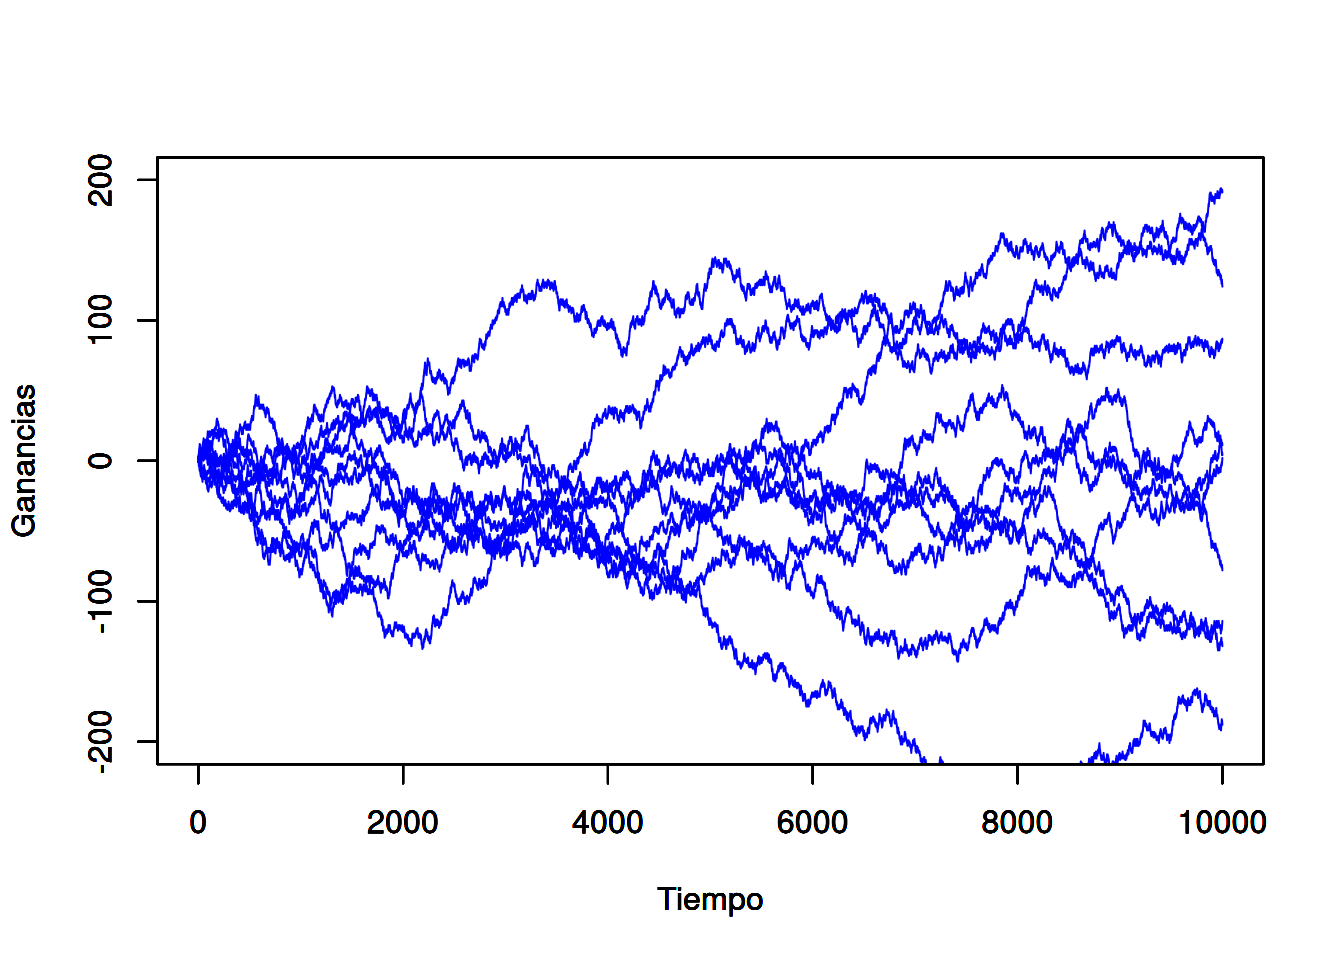
\includegraphics[width=7in,height=\textheight]{index_files/figure-html/fig31-1.png}

}

\end{figure}%

\subsection{Función de
autocorrelación}\label{funciuxf3n-de-autocorrelaciuxf3n}

Para ampliar la discusión, es posible calcular la fuerza o intensidad de
la dependencia de las variables aleatorias dentro de un proceso
estocástico, ello mediante el uso de las autocovarianzas. Cuando las
covarianzas son normalizadas respecto de la varianza, el resultado es un
término que es independiente de las unidad de medida aplicada, y se
conoce como la \textit{función de autocorrelación}.

Para procesos estacionarios, dicha función de autocorrelación esta dada
por:

\[
\rho(\tau) = \frac{\mathbb{E}[(X_t - \mu)(X_{t+\tau} - \mu)]}{\mathbb{E}[(X_t - \mu)^2]} = \frac{\gamma(\tau)}{\gamma(0)} 
\]

Donde \(\tau = \ldots, -2, -1, 0, 1, 2, \ldots\). Dicha función tiene
las siguientes propiedades:

\begin{enumerate}
\def\labelenumi{\arabic{enumi}.}
\tightlist
\item
  \(\rho(0) = 1\). Es fácil demostrar que la función \(\rho(0)\) es:
\end{enumerate}

\[
\rho(0) = \frac{\mathbb{E}[(X_t - \mu)(X_{t + 0} - \mu)]}{\mathbb{E}[(X_t - \mu)^2]} = \frac{\mathbb{E}[(X_t - \mu)^2]}{\mathbb{E}[(X_t - \mu)^2]} = 1
\]

\begin{enumerate}
\def\labelenumi{\arabic{enumi}.}
\tightlist
\item
  \(\rho(\tau) = \rho(-\tau)\). Partiendo de la definción de
  \(\rho(\tau)\) podemos ver que la distancia que existe entre \(t\) y
  \(t + \tau\) es \(\tau\), de esta forma la autocorrelación de la
  variable \(X\) entre los periodos antes señalados debería ser la misma
  para el caso en que \(\rho(-\tau)\). Partamos de la ecuación para ver
  más claramente:
\end{enumerate}

\[
\rho(\tau) = \frac{\mathbb{E}[(X_t - \mu)(X_{t + \tau} - \mu)]}{\mathbb{E}[(X_t - \mu)^2]} = \frac{\mathbb{E}[(X_t - \mu)(X_{t - \tau} - \mu)]}{\mathbb{E}[(X_t - \mu)^2]} = \rho(-\tau)
\]

\begin{enumerate}
\def\labelenumi{\arabic{enumi}.}
\tightlist
\item
  \(\abs{\rho(\tau)} \leq 1\), para todo \(\tau\).
\end{enumerate}

Derivado de las propiedades 1 y 2 antes descritas se puede concluir que
sólo es necesario conocer la función de autocorrelación para el caso de
\(\tau = 1, 2, 3, \ldots\), ya que de estos casos podemos derivar los
valores de la función de autocorrelación complementarios de
\(\tau = \ldots, -3, -2, -1\).

Partiendo de los supuestos de ergodicidad en relación a la media,
varianza y covarianzas de un proceso estacionario, podemos estimar
dichos paramétros con las siguientes formulaciones o propuestas de
estimadores puntuales:

\[
\hat{\mu} = \frac{1}{T} \sum^T_{t=1} X_t
\]

\[
\hat{\gamma}(0) = \frac{1}{T} \sum^T_{t=1} (X_t - \hat{\mu})^2 = \hat{\sigma}^2
\]

\[
\hat{\gamma}(\tau) = \frac{1}{T} \sum^{T - \tau}_{t=1} (X_t - \hat{\mu})(X_{t+\tau} - \hat{\mu}) \mbox{, para } \tau = 1, 2, \ldots, T-1
\]

No hacemos la demostración en estas notas --sería deseable que el alumno
revisará la afimación-- pero estos últimos son estimadores consistentes
de \(\mu\), \(\gamma(0)\) y \(\gamma(\tau)\). Por su parte, un estimador
consistente de la función de autocorrelación estará dado por:

\begin{equation}\phantomsection\label{eq-Eq_AutoCorr}{
\hat{\rho}(\tau) = \frac{\sum^{T - \tau}_{t=1} (X_t - \hat{\mu})(X_{t+\tau} - \hat{\mu})}{\sum^T_{t=1} (X_t - \hat{\mu})^2} = \frac{\hat{\gamma}(\tau)}{\hat{\gamma}(0)} \mbox{, para } \tau = 1, 2, \ldots, T-1
}\end{equation}

El estimador de la ecuación (\textbf{?@eq-AutoCorr}) es asintóticamente
insesgado. Por ejemplo, para el caso de un proceso de ruido blanco o
caminata aleatoria, su varianza puede ser aproximada por el valor dado
\(1/T\). Ésta tiene, asintóticamente, una distribución normal. Dado
esto, el intervalo de confianza al \(95\%\) será el dado por
\(\pm 2/\sqrt{T}\), en el cual se encuentra la mayoría de los
coeficientes de autocorrelación estimados.

Ahora discutamos algunos ejemplos o aplicaciones. Cuando se realiza la
evaluación de la estimación de un modelo de series de tiempo es
importante saber si los residuales del modelo realmente tienen
propiedades de un proceso puramente aleatorio, en partícular, si ellos
no están correlacionados entre sí. Así, la hipotésis a probar será:

\[
H_0 : \rho(\tau) = 0 \mbox{, para todo } \tau = 1, 2, \ldots, m \mbox{ y } m < T
\]

Esta expresión se puede interpretar como una prueba respecto de si la
correlación entre la información de periodos atrás es cero con la
información contemporánea. Para hacer una pruena global de la hipotésis
de sí un número \(m\) de coeficientes de autocovarianzas son cero Box y
Pierce (1970) desarrollarón la siguiente estadística:

\[
Q^* = T \sum_{j = 1}^{m} \hat{\rho} (j)^2
\]

Bajo la hipotésis nula esta estadística se distribulle asintóticamente
como una chi cuadrado (\(\chi^2\)) con \(m-k\) grados de libertad y con
\(k\) que representa al número de paramétros estimados.

Haciendo una aplicación estricta de la distribución de esta estadística,
sabemos que esta se mantiene asintóticamente. Greta, Ljung y Box (1978)
propusieron la siguiente modificación de la estadística para muestras
pequeñas:

\[
Q = T(T + 2) \sum_{j = 1}^{m} \frac{\hat{\rho} (j)^2}{T - j}
\]

La cual también se distribulle asintóticamente como \(\chi^2\) con
\(m-k\) grados de libertad.

También es intuitivamente claro que la hipótesis nula de no
autocorrelación de residuales debería ser rechazada si alguno de los
valores \(\hat{\rho} (j)\) es muy grande, es decir, si \(Q\) o \(Q^*\)
es muy grande. O más precisamente, si estas estadísticas son más grandes
que los correspondientes valores críticos de la distribución \(\chi^2\)
con \(m-k\) grados de libertad a algún grado dado de signficancia.

Una alternativa para esta prueba es una del tipo Multiplicadores de
Lagrange (o LM) desarrollada por Breusch (1978) y Godfrey (1978). La
cual, al igual que las estadísticas \(Q\) y \(Q^*\), la hipotesis nula
está dada por:

\begin{itemize}
\item
  \(H_0\): Los residuales no están autocorrelacionados.
\item
  \(H_a\): Los residuales muestran alguna acutocorrelación de forma
  autoregresiva o de medias móviles.
\end{itemize}

La prueba consiste en realizar una regresión auxiliar en la cual los
residuales se estiman en función de las variables explicativas del
modelo original y en los residuales mismos pero rezagados hasta el
término \(m\) (regresión auxiliar). La prueba resulta en una estadìstica
con una distribución \(\chi^2\) con \(m\) grados de libertad la cual
está dada por la expresión:

\[
LM = T \times R^2
\]

Donde \(R^2\) es el resultante de la regresión auxiliar y \(T\) es el
número de observaciones totales.

En comparación con una prueba Durbin - Watson que es comúnmente usada en
la econometría tradicional, para probar autocorrelación de los
residuales, las estadísticas \(Q\), \(Q^*\) y \(LM\) tienen las
siguientes ventajas:

\begin{enumerate}
\def\labelenumi{\arabic{enumi}.}
\item
  Permiten corroborar la existencia de autocorrelación para cualquier
  orden, y no solo para un primer orden (es decir, para cualquier valor
  de \(\tau = 1, 2, 3, \ldots\));
\item
  Los resultados se mantienen aún y cuando exista una probable variable
  endógena en forma rezagada, y
\item
  No depende del orden o la forma en que se acomoden las observaciones,
  algo que es muy probalble que ocurra en la econometría tradicional.
\end{enumerate}

El hecho de los residuales no estén autocorrelacionados no implica que
estos sean independientes y normalmente distribuidos. La ausencia de
autocorrelación no implica una independencia estocástica si las
variables son normalmente distribuidas.

A menudo se asume que estos residuales están distribuidos normalmente,
ya que la mayoría de las pruebas estadísticas tienen este supuesto
detrás. No obstante, ello también depende de los otros momentos de la
distribución, específicamente del tercer y cuarto momento. Los cuales
expresan como:

\[
\mathbb{E}[(X_t - \mathbb{E}[X_t])^i] \mbox{, } i = 3, 4
\]

El tercer momento es necesario para determinar el sesgo, el cual esta
dado como:

\[
\hat{S} = \frac{1}{T} \frac{\sum_{t = 1}^{T} (X_t - \hat{\mu})^3}{\sqrt{\hat{\gamma}(0)^3}}
\]

Para distribuciones simetricas (como en el caso de la distribución
normal) el valor teórico para el sesgo es cero.

La curtosis, la cual esta dada en función del cuarto momento, se puede
expresar como:

\[
\hat{K} = \frac{1}{T} \frac{\sum_{t = 1}^{T} (X_t - \hat{\mu})^4}{\hat{\gamma}(0)^2}
\]

Para el caso de una distribución normal, esta estadística toma el valor
de 3. Valores más grandes que 3 indican que la distribución tienen colas
anchas. En tales casos se ubican a los datos financieros.

Usando el valor de las estadísticas para medir el sesgo y la curtosis,
\(S\) y \(K\), respectivamente, Jarque y Bera (1980) propusieron una
prueba de normalidad, la cual puede ser aplicada a series de tiempo en
niveles o en diferencias indistintamente. Dicha prueba se expresa como:

\[
JB = \frac{T}{6} \left(\hat{S} + \frac{1}{4} (\hat{K} - 3)^2 \right) 
\]

La cual tiene una distribución \(\chi^2\) con \(2\) grados de libertad y
donde \(T\) es el tamaño de la muestra. La hipótesis de que las
observaciones están distribuidas de forma normal se rechaza si los
valores de la estadística de prueba es más grande que los
correspondientes valores criticos en tablas.

Veamos un ejemplo para ilustrar el uso de la función de autocorrelación.
Tomemos como variable al número de pasajeros transportados por el
sistema de transporte del metro de la
CDMX.\footnote{Los datos y algoritmo está disponible en el reepositorio de GitHub y corresponde a la Clase 3.}
Los datos empleados fueron tomados del INEGI y son una serie de tiempo
en el periodo que va de enero de 2000 a junio de 2019, es decir, 234
observaciones. Como se puede apreciar en la Figura \ref{Pax_Metro}, el
número de pasajeros por mes ha oscilado significativamente a lo largo de
tiempo. Incluso podemos observar un cambio estructural de la serie entre
2011 y 2012. Asimismo, podemos ubicar una caida atípica que ocurrió en
septiembre de 2017.

\begin{figure}
  \centering
  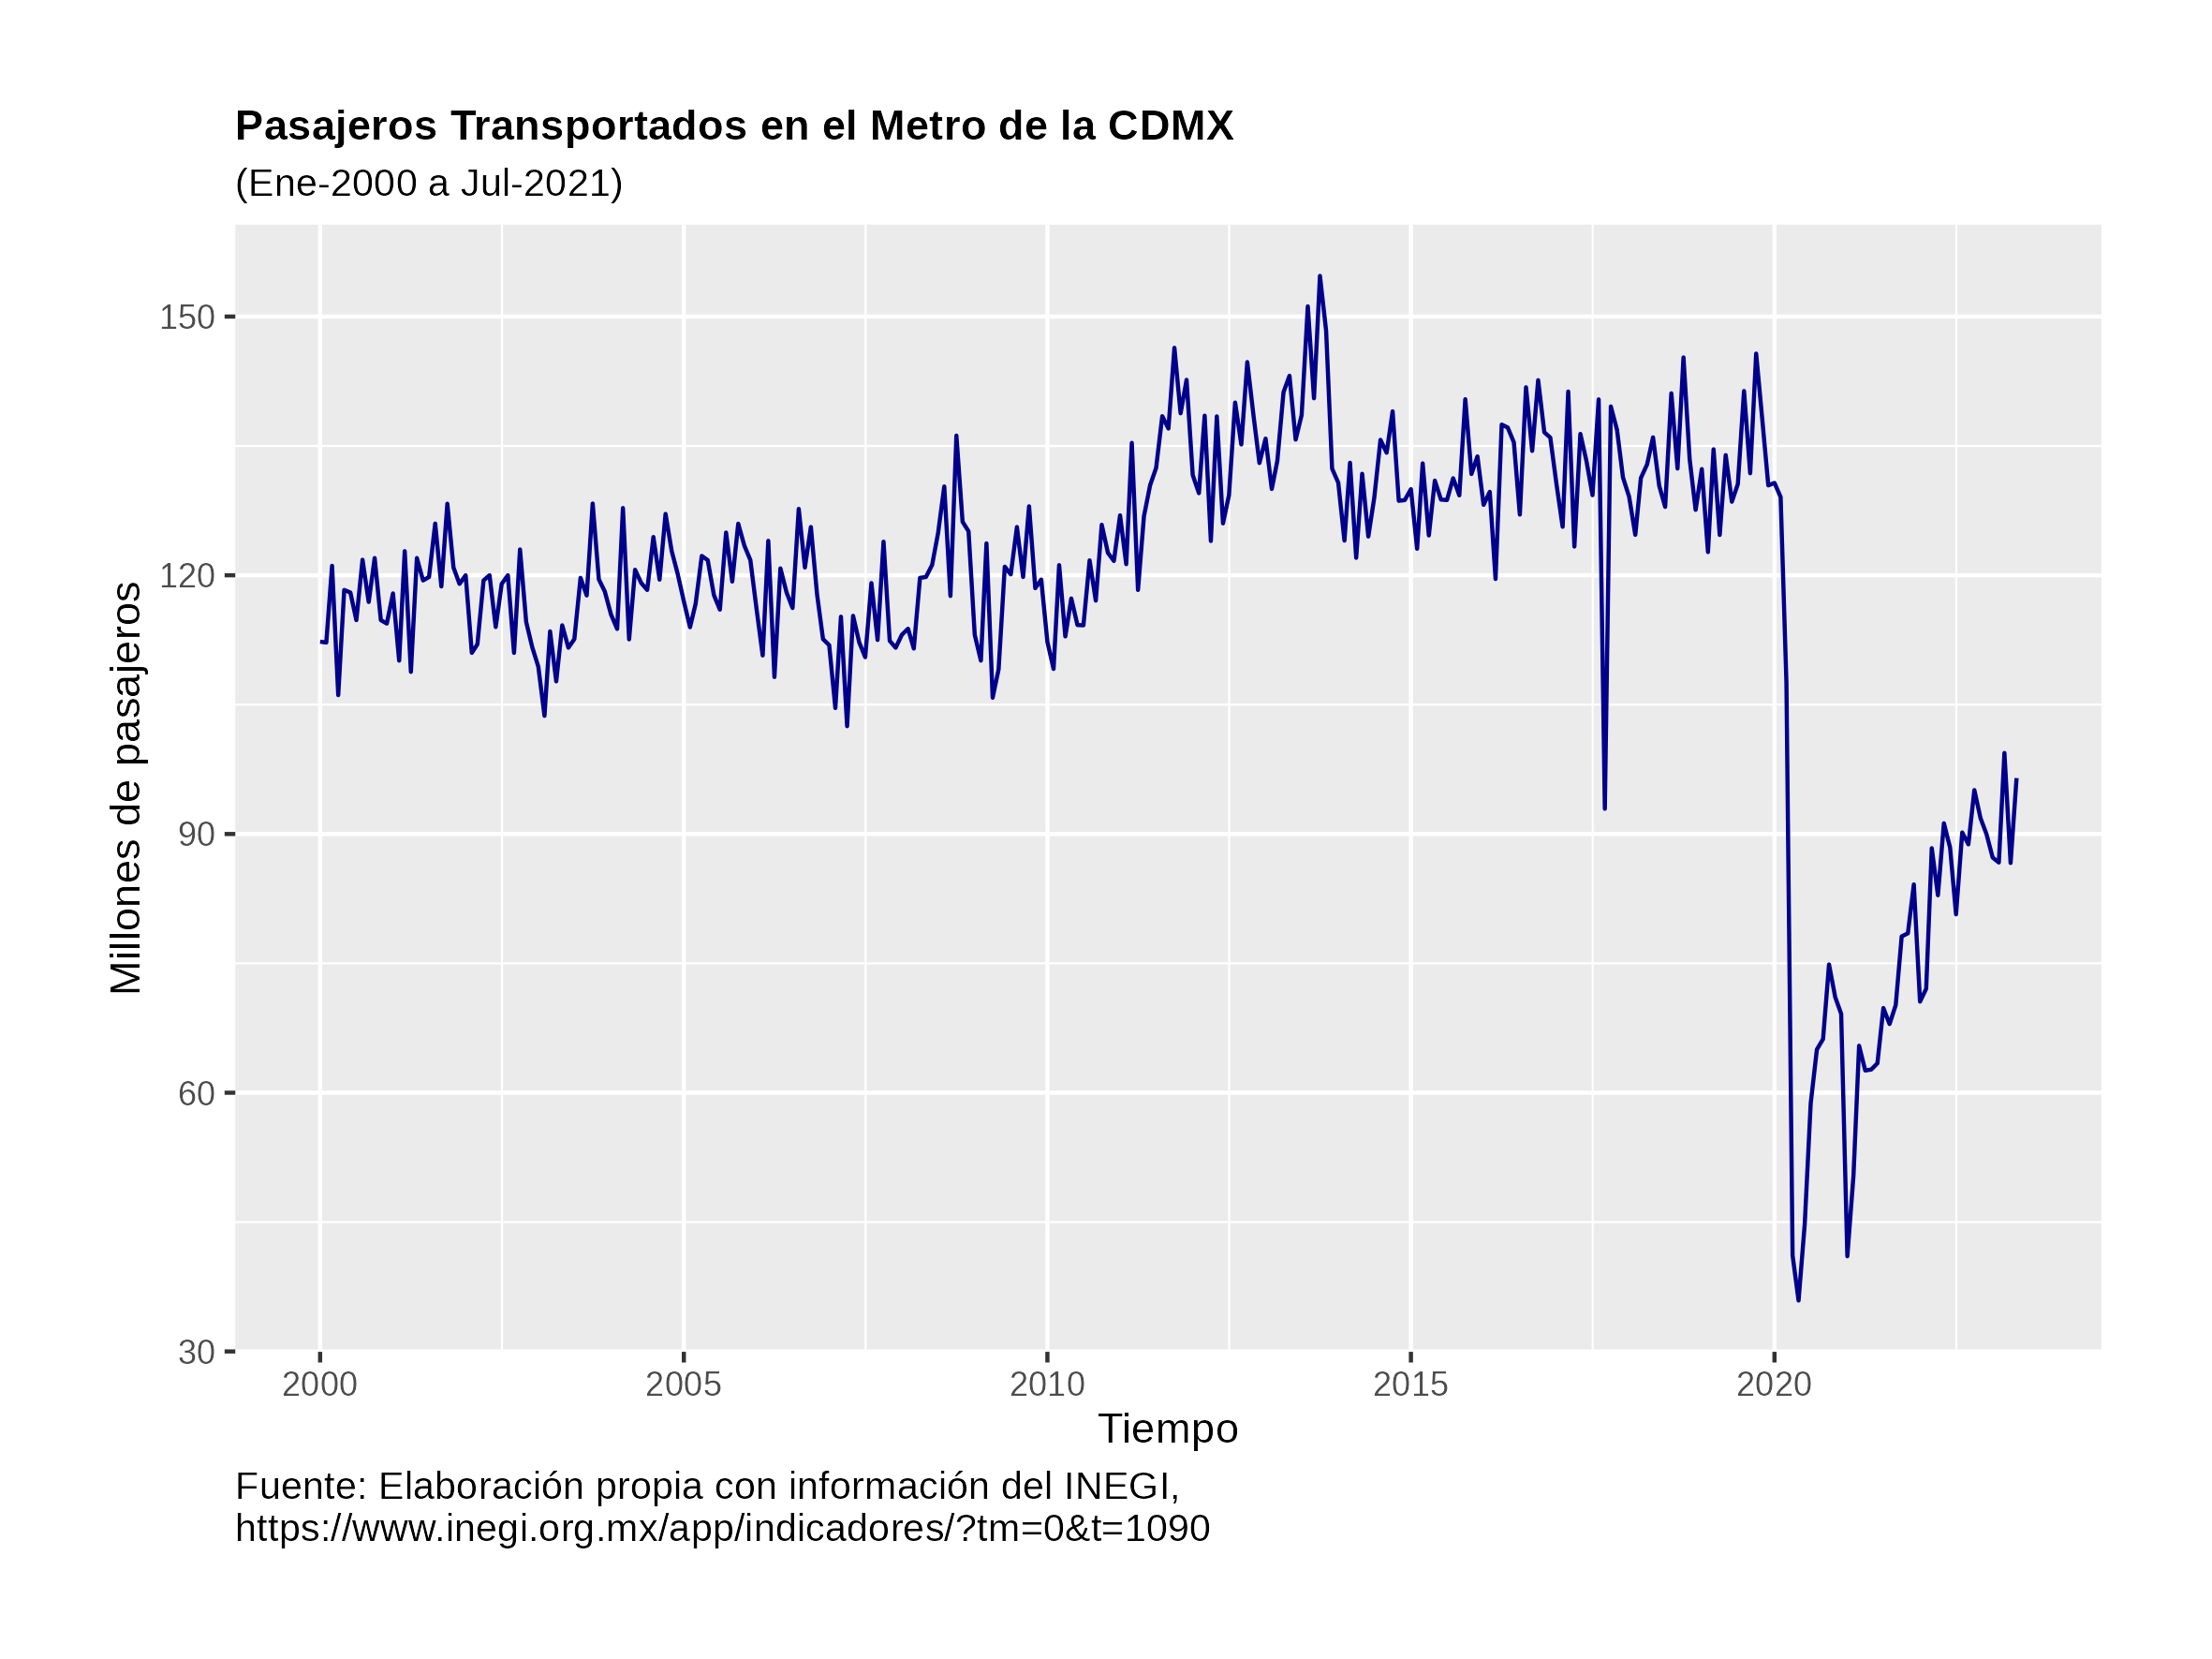
\includegraphics[width=1.0\textwidth]{Pax_Metro}
  \caption{Evolución del número de pasajeros en el Metro de la CDMX, enero de 2000 a junio de 2019}
  \label{Pax_Metro}
\end{figure}

A esta serie de tiempo le calculamos los pincipales estadísticos hasta
ahora estudiados y obtenemos el Cuadro \ref{Est_Pax}. En dicho cuadro se
destaca que se muestra la función de autocirrelación para los tres
primeros rezagos. Para mayor detalle, en la Figura \ref{Correlograma} se
muestra la función de autocorrelación, en donde las bandas descritas por
las líneas azules son el intervalo de confianza desntro de las cuales no
se puede rechazar la hipotésis nula de que \(H_0: \hat{\rho}(p) = 0\),
para todo \(\tau = 1, 2, \ldots, T-1\).

\begin{longtable}[]{@{}
  >{\raggedright\arraybackslash}p{(\columnwidth - 2\tabcolsep) * \real{0.7778}}
  >{\raggedright\arraybackslash}p{(\columnwidth - 2\tabcolsep) * \real{0.2222}}@{}}
\caption{Estadísticas descriptivas del número de pasajeros en el Metro
de la CDMX, enero de 2000 a junio de 2019}\tabularnewline
\toprule\noalign{}
\begin{minipage}[b]{\linewidth}\raggedright
Estadística
\end{minipage} & \begin{minipage}[b]{\linewidth}\raggedright
Valor
\end{minipage} \\
\midrule\noalign{}
\endfirsthead
\toprule\noalign{}
\begin{minipage}[b]{\linewidth}\raggedright
Estadística
\end{minipage} & \begin{minipage}[b]{\linewidth}\raggedright
Valor
\end{minipage} \\
\midrule\noalign{}
\endhead
\bottomrule\noalign{}
\endlastfoot
\(\hat{\mu} = \frac{1}{T} \sum^T_{t=1} X_t\) & 124.3000 \\
\(\hat{\gamma}(0) = \frac{1}{T} \sum^T_{t=1} (X_t - \hat{\mu})^2\) &
103.6400 \\
\(\hat{\gamma}(1) = \frac{1}{T} \sum^{T - 1}_{t=1} (X_t - \hat{\mu})(X_{t+1} - \hat{\mu})\)
& 63.1100 \\
\(\hat{\gamma}(2) = \frac{1}{T} \sum^{T - 2}_{t=1} (X_t - \hat{\mu})(X_{t+2} - \hat{\mu})\)
& 72.9100 \\
\(\hat{\gamma}(3) = \frac{1}{T} \sum^{T - 3}_{t=1} (X_t - \hat{\mu})(X_{t+3} - \hat{\mu})\)
& 63.6900 \\
\(\hat{\rho}(1) = \frac{\sum^{T - 1}_{t=1} (X_t - \hat{\mu})(X_{t+1} - \hat{\mu})}{\sum^T_{t=1} (X_t - \hat{\mu})^2} = \frac{\hat{\gamma}(1)}{\hat{\gamma}(0)}\)
& 0.6089 \\
\(\hat{\rho}(2) = \frac{\sum^{T - 2}_{t=1} (X_t - \hat{\mu})(X_{t+2} - \hat{\mu})}{\sum^T_{t=1} (X_t - \hat{\mu})^2} = \frac{\hat{\gamma}(2)}{\hat{\gamma}(0)}\)
& 0.7035 \\
\(\hat{\rho}(3) = \frac{\sum^{T - 3}_{t=1} (X_t - \hat{\mu})(X_{t+3} - \hat{\mu})}{\sum^T_{t=1} (X_t - \hat{\mu})^2} = \frac{\hat{\gamma}(3)}{\hat{\gamma}(0)}\)
& 0.6145 \\
\(Q^* = T \sum_{j = 1}^{1} \hat{\rho} (j)^2\) & 86.7577 \\
\(Q^* = T \sum_{j = 1}^{2} \hat{\rho} (j)^2\) & 290.9279 \\
\end{longtable}

label\{Est\_Pax\}

\begin{figure}
  \centering
  \includegraphics[width = 0.8\textwidth]{ACF_Metro}
  \caption{Función de Autocorrelación: 150 rezagos del número de pasajeros en el Metro de la CDMX, enero de 2000 a junio de 2019}
  \label{Correlograma}
\end{figure}


\printbibliography


\end{document}
